% !TEX encoding = UTF-8
% !TEX TS-program = pdflatex
% !TEX root = ../tesi.tex

%**************************************************************
\chapter{Progettazione e codifica}
\label{cap5}
%**************************************************************

\section{Design dell'interfaccia grafica}
\label{sec:design-gui}
Per definire un primo design dell'interfaccia grafica sono stati realizzati alcuni \gls{mock up}, utili anche per semplificare la progettazione e l'analisi dei vari aspetti relativi all'esperienza dell'utente.
Come da requisiti l'interfaccia è stata sviluppata in modalità "wizard", ovvero una procedura a fasi dove l'utente deve completare l'azione richiesta in una fase per poter passare alla successiva.

Sono state individuate 3 fasi differenti (a cui corrispondono 3 pagine dell'interfaccia grafica), di seguito definite:

\begin{itemize}
\item La fase di \textit{training}: corrisponde alla prima fase, in cui viene creato il process model tramite tecniche di Machine Learning. Viene utilizzato l'event log caricato dall'utente contenente tracce complete. L'utente potrà procedere alla fase successiva solo se il process model è stato generato con successo;

\item La fase di \textit{runtime}: corrisponde alla seconda fase, in cui vengono generate le raccomandazioni. Viene utilizzato l'event log caricato dall'utente contenente tracce incomplete. L'utente potrà procedere solo se il processo di generazione delle raccomandazioni termina con successo;

\item La fase di visualizzazione: corrisponde alla terza ed ultima fase, in cui l'utente può visualizzare le raccomandazioni generate e le corrispettive spiegazioni. Questa fase rappresenta l'obiettivo finale dell'interfaccia, e la più "interessante" dal punto di vista dell'utente, che ha superato le fasi precedenti con lo scopo di visualizzare le raccomandazione e spiegazioni a cui era interessato.

\end{itemize}

Con il termine \textbf{esperimento} ci si riferirà, nel resto del testo, ad una singola esecuzione completa di almeno la prima fase.

\subsection{Fase di training}

\begin{figure}[H] 
    \centering 
    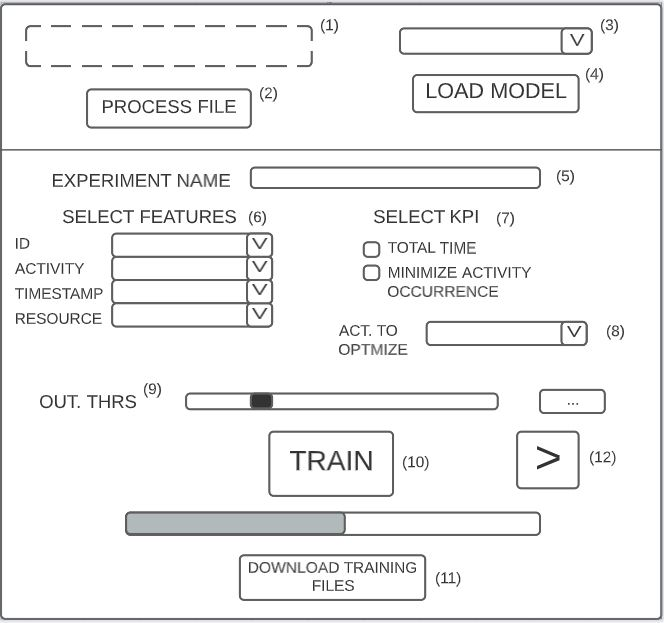
\includegraphics[width=0.9\columnwidth]{immagini/mockup-train.jpg} 
    \caption{Design iniziale della pagina relativa alla fase di training}
    \label{fig:mockup-train}
\end{figure}

In \autoref{fig:mockup-train} il mock up su cui si è basato l'aspetto finale della pagina relativa alla fase di training.
\\
Seguendo i requisiti il flusso principale di utilizzo della pagina è il seguente (i riferimenti numerici successivi, in forma (x), sono relativi alla \autoref{fig:mockup-train}):

\begin{enumerate}
\item L'utente carica l'event log che vuole utilizzare per il processo di training, usando l'area di drag-and-drop (1) e clicca il pulsante "Process file" (2) che permette all'interfaccia di analizzare ed elaborare il file caricato;

\item L'utente dichiara i nomi delle colonne dell'event log caricato, corrispondenti alle features richieste, usando gli elementi dropdown (6), le opzioni disponibili sono l'insieme delle colonne dell'event log caricato (grazie alla fase di elaborazione), questo semplifica il processo, in quanto l'utente deve solo selezionare la colonna giusta al posto di scriverla, riducendo gli errori e velocizzando la compilazione. Da notare come le features sono tutte obbligatorie tranne la feature "resource";

\item L'utente seleziona il KPI che desidera (7), se sceglie "Minimize activity occurrence" dovrà anche dichiarare il nome dell'attività da ottimizzare, tramite l'apposito dropdown (8), che anche qui semplifica e velocizza la compilazione in quanto contiene già l'insieme di tutte le attività presenti nell'event log;

\item L'utente inserisce il nome dell'esperimento nella casella di testo (5) apposita e seleziona, tramite uno slider (9), la soglia degli outliers che desidera (essa ha comunque un valore di default iniziale);

\item L'utente avvia il processo di training cliccando sul pulsante "Train" (10);

\item Al termine del processo di training l'utente può, se lo desidera, scaricare i file che compongono il process model cliccando il pulsante "Download training files" (11); 

\item Infine l'utente può passare alla pagina successiva cliccando sul pulsante a freccia (12).

\end{enumerate}

Va evidenziato che lo step 4. pu essere effettuato in qualsiasi momento, basta che sia prima del passo 5. e dopo il passo 1., mentre il passo 6. è opzionale. 
\\ \\
Se è già presente un process model (creato in un esperimento precedente) è possibile caricarlo nel sistema e saltare tutto il processo di training (che può richiedere una quantità d tempo considerevole). Il flusso di esecuzione alternativo è il seguente (i riferimenti numerici successivi, in forma (x), sono relativi alla \autoref{fig:mockup-train}):

\begin{enumerate}
\item L'utente seleziona un process model già creato tra quelli disponibili, usando l'apposito dropdown (3) e clicca il pulsante "Load model" (4) per caricare il process model nel sistema;

\item L'utente può, se lo desidera, scaricare i file che compongono il process model cliccando il pulsante "Download training files" (11); 

\item Infine l'utente può passare alla pagina successiva cliccando sul pulsante a freccia (12).

\end{enumerate}

In questo caso invece, il passo 2. è da considerarsi opzionale.


\subsection{Fase di runtime}

\begin{figure}[!h] 
    \centering 
    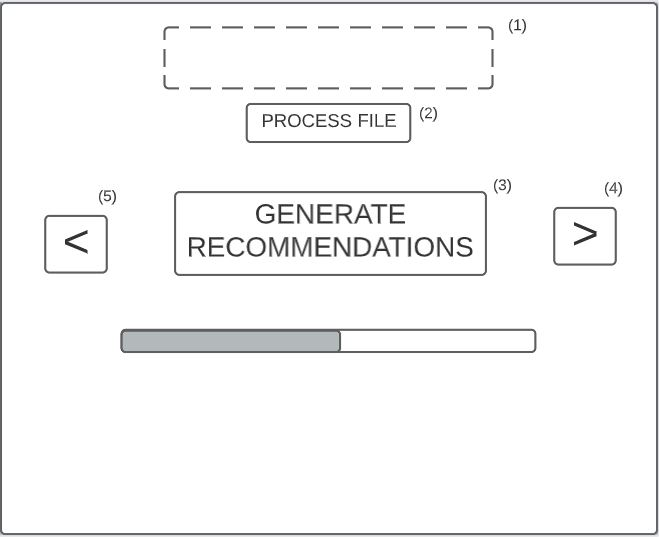
\includegraphics[width=0.8\columnwidth]{immagini/mockup-run.jpg} 
    \caption{Design iniziale della pagina relativa alla fase di runtime}
    \label{fig:mockup-run}
\end{figure}

In \autoref{fig:mockup-run} il mock up su cui si è basato l'aspetto finale della pagina relativa alla fase di runtime.
\\
Seguendo i requisiti il flusso principale di utilizzo della pagina è il seguente (i riferimenti numerici successivi, in forma (x), sono relativi alla \autoref{fig:mockup-run}):

\begin{enumerate}

\item L'utente carica l'event log che vuole utilizzare per la generazione delle raccomandazioni, usando l'area di drag-and-drop (1) e clicca il pulsante "Process file" (2) che permette all'interfaccia di analizzare ed elaborare il file caricato;

\item L'utente clicca sul pulsante "Generate recommendations" (3) per avviare il processo di generazione delle raccomandazioni;

\item Al termine del processo di generazione delle raccomandazioni l'utente può passare alla pagina successiva cliccando sul pulsante a freccia (4).

\end{enumerate}


\subsection{Fase di visualizzazione}

\begin{figure}[!h] 
    \centering 
    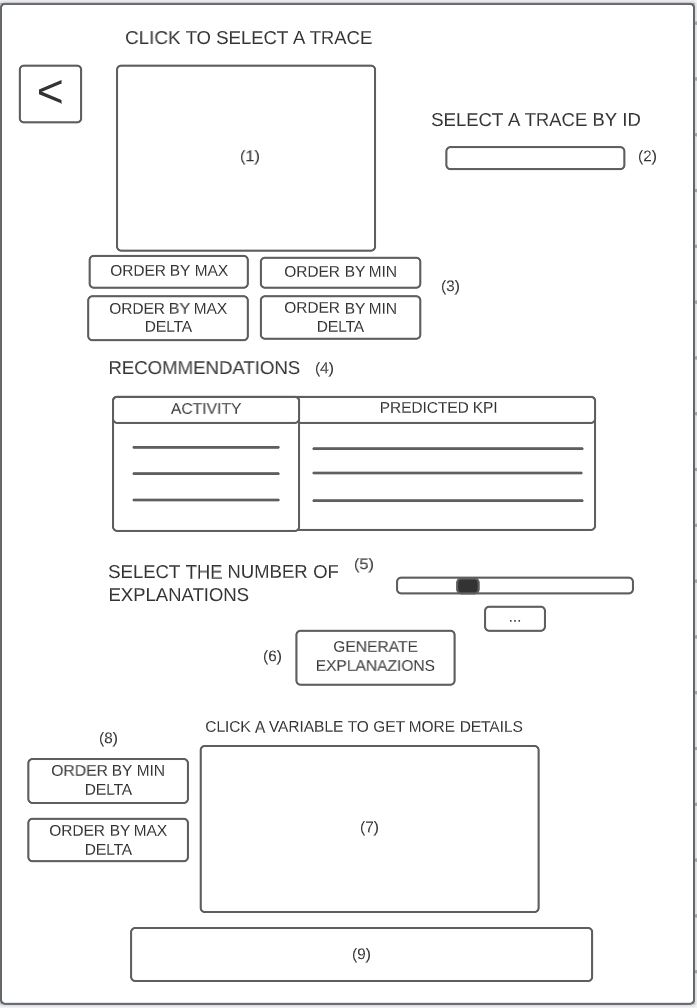
\includegraphics[width=0.7\columnwidth]{immagini/mockup-explain.jpg} 
    \caption{Design iniziale della pagina relativa alla fase di visualizzazione}
    \label{fig:mockup-explain}
\end{figure}

In \autoref{fig:mockup-explain} il mock up su cui si è basato l'aspetto finale della pagina relativa alla fase di visualizzazione.
\\
Seguendo i requisiti il flusso principale di utilizzo della pagina è il seguente (i riferimenti numerici successivi, in forma (x), sono relativi alla \autoref{fig:mockup-explain}):

\begin{enumerate}
\item L'utente visualizza, tramite il grafico (1), le raccomandazioni generate, e ha la possibilità di selezionare una traccia cliccando sulla rispettiva raccomandazione nel grafico oppure inserendo la traccia nella casella di testo apposita (2);

\item L'utente, se desidera, può riordinare le raccomandazioni generate usando uno dei 4 pulsanti in (3);

\item Una volta selezionata la traccia l'utente può visualizzare fino ad un massimo di 3 raccomandazioni, con relativo KPI predetto nella tabella (4);

\item L'utente può selezionare una delle raccomandazioni di cui vuole visualizzare la spiegazione, tramite un click sulla corrispondente riga della tabella (4);

\item L'utente può scegliere la quantità di variabili da visualizzare nella spiegazione tramite lo slider apposito (5), in ogni caso viene definita una quantità di default;

\item L'utente avvia il processo di generazione della spiegazione cliccando sul pulsante "Generate explanazions" (6);

\item Al termine del processo di generazione della spiegazione l'utente può visualizzarla nel grafico apposito (7);

\item L'utente, se desidera, può riordinare le variabili della spiegazione generata usando uno dei 2 pulsanti in (8);

\item L'utente può cliccare su una specifica variabile della spiegazione generata per ottenere maggiori dettagli in formato testuale nello spazio designato (9).

\end{enumerate}





\section{Architettura del sistema}
L'architettura del sistema segue il \textit{design pattern} \textbf{MVP}, molto comune per lo sviluppo di interfacce grafiche. 


\begin{figure}[H] 
    \centering 
    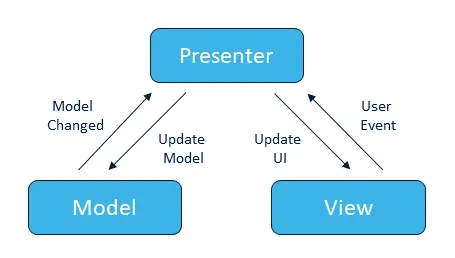
\includegraphics[width=0.9\columnwidth]{immagini/mvp.png} 
    \caption{Struttura design pattern MVP \cite{site:mvp}}
    \label{fig:mvp}
\end{figure}

Esso è composto da 3 componenti principali:

\begin{itemize}

\item \textit{Model}: Contiene la logica di business, ovvero i dati a cui siamo interessati, ed è responsabile della loro gestione (lettura, scrittura, modifica);

\item \textit{View}: Rappresenta l'interfaccia più a stretto contatto con l'utente e si occupa di mostrare i dati e di raccogliere l'input dell'utente. Nel caso particolare del MVP, la vista è passiva, quindi non dovrebbe contenere nessuna logica applicativa ma solo visuale;

\item \textit{Presenter}: Rappresenta il ponte do comunicazione tra View e Model, riceve gli input dalla View, si occupa di recuperare i dati e dell'esecuzione della logica di business da parte del Model per poi formattare e inviare alla View i dati da visualizzare.

\end{itemize}

Un'aspetto importante è il fatto che la View non ha conoscenze (e nessun a dipendenza) dal Model e viceversa. 
\\
Questo porta ai principali motivi che hanno spinto a scegliere il design pattern:

\begin{itemize}

\item Testabilità: le singole parti possono essere testate in isolamento più facilmente dato che le logiche applicative e visuali sono separate;

\item Separazione dei compiti: la separazione logiche e la ridotta dipendenza tra le parti (in particolare Model e View sono totalmente separati) permette di avere codice più modulare, quindi semplice e mantenibile;

\item Compatibilità con il framework: vista la forma dichiarativa delle viste costruite con il framework Dash si adatta bene alla View passiva caratteristica del MVP.

\end{itemize}

\section{Progettazione classi dell'interfaccia grafica}
Di seguito saranno utilizzati i digrammi \gls{UML} per la rappresentazione delle classi che compongono l'interfaccia.

\subsection{Progettazione View}
\label{subsec:prog-views}
Per la progettazione della componente View è stata sviluppata una struttura a views multiple, una per ogni pagina descritta nella \autoref{sec:design-gui}.

\begin{figure}[H] 
    \centering 
    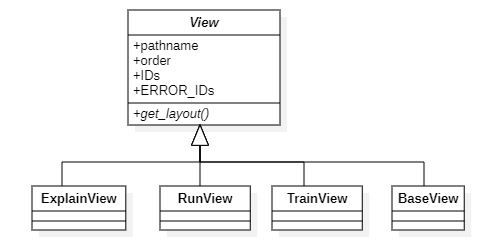
\includegraphics[width=0.8\columnwidth]{immagini/uml-views.jpg} 
    \caption{Diagramma UML per la classi della View}
    \label{fig:uml-views}
\end{figure}

Viene definita una classe astratta, che rappresenta una view generica, sulla quale si basano le altre views. Questo è utile per esporre le funzionalità comuni che deve avere una view.
In particolare ogni view deve definire:

\begin{itemize}

\item Un attributo \texttt{pathname} che rappresenta il nome della vista, usato per sviluppare l'interfaccia in modalità wizard;

\item Un attributo \texttt{order} che rappresenta l'ordimento utilizzato per mostrare le pagine, serve a definire i predecessori e/o successori di ogni pagina, usato per sviluppare l'interfaccia in modalità wizard;

\item Un attributo \texttt{IDs} che definisce l'insieme di tutti gli identificativi univoci dei componenti usati dal framework Dash per la costruzione della parte grafica dell'interfaccia; 

\item Un attributo \texttt{ERROR\_IDs} che definisce l'insieme di tutti gli identificativi univoci dei componenti usati dal framework Dash per visualizzare gli eventuali messaggi d'errore; 

\item L'implementazione del metodo astratto \texttt{get\_layout} che definisce l'insieme dei componenti Dash e la loro struttura per la creazione della parte grafica della specifica pagina.

\end{itemize}

Sono state definite 4 classi concrete che implementano la classe \texttt{View}:
\begin{itemize}
\item La classe \texttt{TrainView} relativa alla pagina per la fase di training, 
\item La classe \texttt{RunView} relativa alla pagina per la fase di runtime, 
\item La classe \texttt{ExplainView} relativa alla pagina per la fase di visualizzazione e 
\item La classe \texttt{BaseView} che si occupa della gestione dei componenti comuni a tutte le view (ad esempio i pulsanti per navigare tra le pagine).
\end{itemize}


\subsection{Progettazione Model}
La progettazione del Model ha tenuto conto del back-end sottostante, cercando di suddividere la struttura in classi specializzate, promuovendo l'incapsulamento e la modularità.

\begin{figure}[H] 
    \centering 
    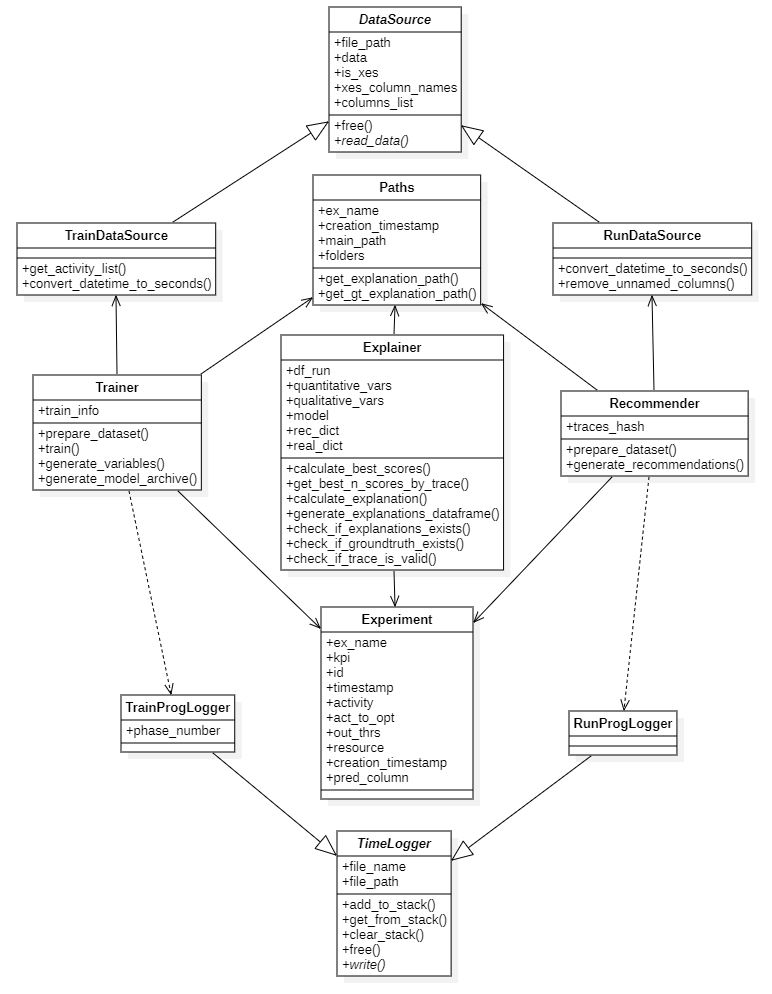
\includegraphics[width=1\columnwidth]{immagini/uml-model.jpg} 
    \caption{Diagramma UML per la classi del Model}
    \label{fig:uml-model}
\end{figure}



Del diagramma di classi in \autoref{fig:uml-model} si possono individuare le 3 classi principali, le cui responsabilità sono correlate alle 3 fasi descritte nella \autoref{sec:design-gui}:

\begin{itemize}
\item La classe \texttt{Trainer} che gestisce il processo di training e la memorizzazione i dati generati, in particolare sfrutta il metodo \texttt{prepare\_dataset} che si occupa di processare l'event log caricato per prepararlo al processo di training ed il metodo \texttt{train} che esegue il processo di training stesso per generare il process model;


\item La classe \texttt{Recommender} che gestisce il processo di generazione e memorizzazione delle raccomandazioni. Anche per questa classe è necessario il metodo \texttt{prepare\_dataset} per processare l'event log caricato dall'utente e renderlo utilizzabile per il processo di generazione delle raccomandazioni che, a sua volta, viene eseguito dal metodo \texttt{generate\_recommendations};

\item La classe \texttt{Explainer} che si occupa della generazione e gestione e memorizzazione delle spiegazioni per le raccomandazioni. Per far questo utilizza i dati prodotti dalle classi sopra descritte (ad esempio l'attributo \texttt{model} che rappresenta il process model generato) ed il metodo \texttt{calculate\_explanations} che genera le spiegazioni per una singola raccomandazione. Inoltre si occupa della visualizzazione delle raccomandazioni, generando le struttura dati che userà poi il componente View, usando i metodi \texttt{calculate\_best\_scores} e \texttt{get\_best\_n\_scores};

\end{itemize}

Le classi principali sopra descritte sfruttano a loro volta delle classi accessorie che si occupano di quelle funzionalità che pur rimanendo necessarie possono essere separate da quello che è il compito della classe principale. Esse sono:

\begin{itemize}
\item La classe \texttt{TrainDataSource} che viene usata dalla classe \texttt{Trainer} per la gestione dell'event log, infatti rappresenta la sorgente dei dati per il processo di training. Deriva dalla classe astratta \texttt{DataSource} di cui implementa il metodo \texttt{read\_data} che si occupa di leggere il file dell'event log dalla memoria. Alcuni attributi di nota sono, ad esempio, \texttt{data} che contiene i dati dell'event log in forma grezza e \texttt{columns\_list} che contiene tutti i nomi delle colonne presenti nell'event log. Offre i metodi \texttt{get\_activity\_list} per ottenere la lista di attività presenti nell'event log (dopo aver dichiarato la feature "activity") ed il metodo \texttt{convert\_datetime\_to\_seconds} per convertire i dati temporali della colonna relativa alla feature "timestamp" in secondi;

\item La classe \texttt{RunDataSource} che rappresenta la sorgente di dati, relativi all'event log, per la classe \texttt{Recommender}. Essa ha la sua implementazione del metodo \texttt{read\_data} per la lettura del file dell'event log in memoria. Gli scopi sono paralleli a quelli della classe \texttt{TrainDataSource} e gli attributi hanno funzioni simili. Una differenza è rappresentata dal metodo \texttt{remove\_unnamed\_columns} che ripulisce l'event log di eventuali colonne vuote o senza identificativo che possono generarsi dopo aver letto i dati con il metodo \texttt{read\_data};

\item La classe \texttt{Experiment} è una classe senza metodi che contiene tutti i dati relativi all'esperimento corrente, ed esempio \texttt{ex\_name} identifica il nome dell'esperimento, \texttt{creation\_timestamp} il timestamp della creazione dell'esperimento mentre \texttt{id}, \texttt{timestamp}, \texttt{activity} e \texttt{resource} rappresentano colonne relative alle varie features richieste per gli event log. La classe viene usata da tutte e 3 le classi principali;

\item La classe \texttt{Paths}, utilizzata da tutte e 3 le classi principali per la gestione di ogni percorso dei vari file usati per la  memorizzazione dei dati generati, così da avere una sorgente univoca e facilitarne l'accesso e la modifica;

\item La classe \texttt{TrainProgLogger} che si occupa di gestire la visualizzazione del progresso del processo di training. Viene utilizzata dal metodo \texttt{train} della classe \texttt{Trainer};

\item La classe \texttt{RunProgLogger} che si occupa di gestire la visualizzazione del progresso del processo di generazione delle raccomandazioni. Viene utilizzata dal metodo \texttt{generate\_recommendations} della classe \texttt{Recommender}.

\end{itemize}


\subsection{Progettazione Presenter}
Per la progettazione del componente Presenter è stato tenuto conto della relazione tra singole view e singolo presenter, è stata definita una struttura a presenter multipli, che va a riflettere la struttura della componente View (\autoref{subsec:prog-views}).


\begin{figure}[H] 
    \centering 
    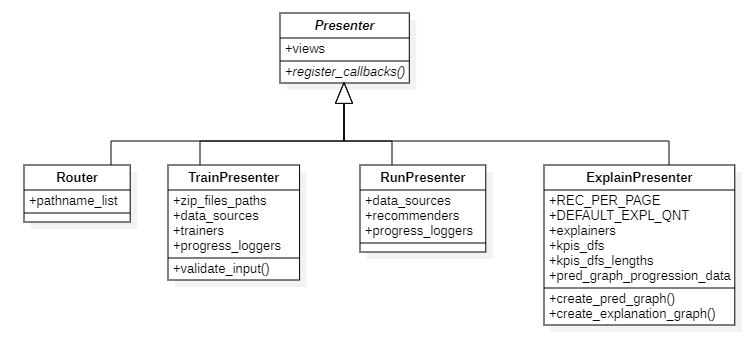
\includegraphics[width=0.8\columnwidth]{immagini/uml-presenters.jpg} 
    \caption{Diagramma UML per la classi del Presenter}
    \label{fig:uml-presenters}
\end{figure}


Anche per progettazione del Presenter è stata sfruttata una classe astratta, la classe \texttt{Presenter}, che espone le funzionalità comuni per un singolo presenter, ovvero: 

\begin{itemize}

\item L'attributo \texttt{views} che contiene i vari riferimenti all'insieme delle view che il presenter può gestire;

\item Il metodo \texttt{register\_callbacks}, un metodo astratto che ogni istanza della classe \texttt{Presenter} deve implementare. Esso definisce tutte le callback che codificano il comportamento dell'interfaccia in risposta all'input dell'utente. Le callback rappresentano lo strumento offerto dal framework Dash per sviluppare la componente interattiva di un'interfaccia grafica.

\end{itemize}

Sono state definite 4 classi concrete che implementano la classe \texttt{Presenter}:

\begin{itemize}
\item La classe \texttt{Router} che gestisce principalmente la classe \texttt{BaseView} della componente View, quindi si occupa di tutti gli aspetti relativi al cambio di pagina. L'attributo \texttt{pathname\_list} è definito in automatico e contiene gli identificativi di tutte le altre view, ordinate secondo il loro attributo \texttt{order}.

\item La classe \texttt{TrainPresenter} che gestisce la classe \texttt{TrainView} della componente View. Si interfaccia con il componente Model per l'esecuzione del processo di training. Per fare questo vengono utilizzati gli attributi \texttt{trainers}, \texttt{data\_sources} e \texttt{progress\_loggers} che rappresentano le istanze delle classi \texttt{Trainer}, \texttt{TrainDataSource} e \texttt{TrainProgLogger} della componente Model. Poiché la pagina della fase di training accetta l'input dell'utente è stato definito il metodo \texttt{validate\_input} che ne gestisce la validazione;

\item La classe \texttt{RunPresenter} che gestisce la classe \texttt{RunView} della componente View. Anche questa classe necessita di interfacciarsi con il componente Model per gestire l'esecuzione del processo di generazione delle raccomandazioni. Sfrutta gli attributi \texttt{recommenders}, \texttt{data\_sources} e \texttt{progress\_loggers} che rappresentano le istanze delle classi \texttt{Recommender}, \texttt{RunDataSource} e \texttt{RunProgLogger} della componente Model.

\item La classe \texttt{ExplainPresenter} che gestisce la classe \texttt{RunView} della componente View. Quindi gestisce la generazione delle spiegazioni, tramite la componente Model, sfruttando, in particolare l'attributo \texttt{explainers} che rappresenta le istanze della classe \texttt{Explainer}. Si occupa anche della visualizzazione delle raccomandazioni e delle spiegazioni, sfruttando il metodo \texttt{create\_pred\_graph} per generare il grafico delle raccomandazioni ed il metodo \texttt{create\_explanation\_graph} per generare il grafico delle spiegazioni. Il resto degli attributi è usato per gestire la visualizzazione dei grafici.

\end{itemize}












 






